\begin{table}[h!]    
	\centering
	\begin{tabular}[12pt]{ |c| c| c|}
    \hline
    \textbf{Variable} & \textbf{Description} & \textbf{Value}\\
	\hline
	$BC$ & Hypotenuse of the triangle & 13 cm\\
	\hline
	$AB$ & Base of the triangle & $x$ cm\\
	\hline
	$AC$ & Altitude of the triangle & $x - 7$ cm\\
	\hline
\end{tabular}
	\caption{}
	\label{tab:10/4/2/5}
\end{table}
	The input parameters are available in \tabref{tab:10/4/2/5}.
Using Baudhayana's theorem,
\begin{align}
	\label{eq:10/4/2/5}
	x^2 + (x - 7)^2 &= 13^2 \\
	\implies    y = x^2 - 7x - 60 &= 0 
\end{align}
which 
 can be expressed as the conic
\begin{align}
    \vec{x}^\top\vec{V}\vec{x} + 2\vec{u}^\top\vec{x} + f = 0 \\
    \vec{V} = \myvec{1 & 0 \\ 0 & 0}, \vec{u} = \myvec{-\frac{7}{2} \\ -\frac{1}{2}}, f = -60.
\end{align}
To find the roots of 
	\eqref{eq:10/4/2/5},
we find the points of intersection of the 
conic 
with the $x$-axis 
\begin{align}
    \vec{x} = \vec{h} + k\vec{m} \\
    \vec{h} = \myvec{0 \\ 0}, \vec{m} = \myvec{1 \\ 0}
\end{align}
using
\eqref{eq:tangent_roots}. 
The values of $k$ are given by
\begin{align}
k_i    &= \frac{1}{1} \brak{\frac{7}{2} \pm \sqrt{\brak{\frac{7}{2}}^2 + 60}} \\
  \implies  k_1 &= -5, k_1 = 12
\end{align}
Hence the points of intersection are
\begin{align}
    \vec{h} + k\vec{m} = \myvec{-5 \\ 0}, \myvec{12 \\ 0}
\end{align}
See 
	\figref{fig:quad1}
Hence the solutions of 
	\eqref{eq:10/4/2/5}
are $x = -5$ and $x = 12$. We reject $x = -5$ as the length of the side
cannot be negative. Hence, the lengths of the sides are
\begin{align}
    AB = 12\ cm \,
    AC = 7\ cm \,
    BC = 13\ cm
\end{align}
See	\figref{fig:quad1}.
\begin{figure}[H]
    \centering
    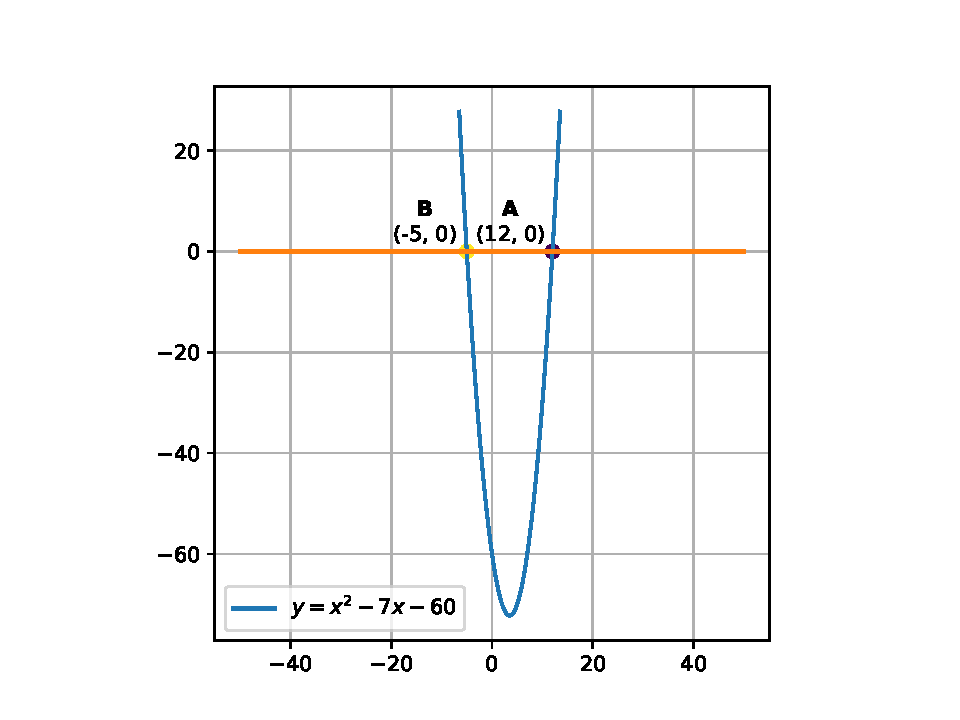
\includegraphics[width=0.75\columnwidth]{chapters/10/4/2/5/figs/parabola.pdf}
    \caption{Intersection of $y = x^2 - 7x - 60$ with the $x$-axis}
	\label{fig:quad1}
\end{figure}
%
\begin{figure}[H]
    \centering
    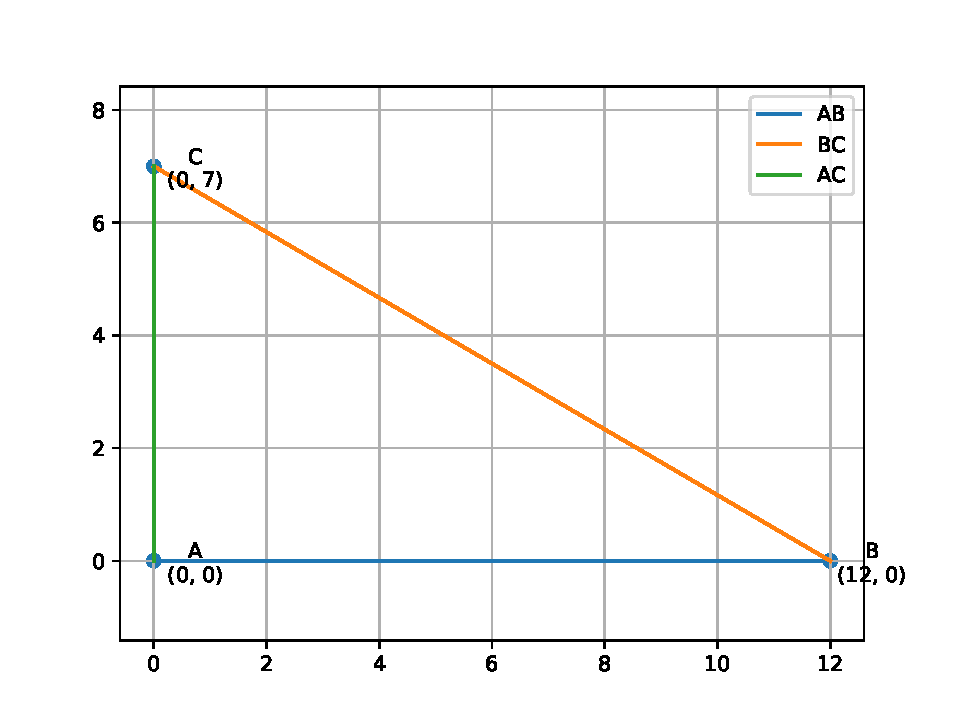
\includegraphics[width=0.75\columnwidth]{chapters/10/4/2/5/figs/triangle.pdf}
    \caption{}
	\label{fig:quad2}
\end{figure}
